\documentclass[10 pt, twoside]{IEEEtran} 
\usepackage{bm}
\usepackage{url}
\usepackage{tikz}
\usepackage{soul}
\usepackage{cite}
\usepackage{color}
\usepackage{pifont}
\usepackage{booktabs}
\usepackage{textcomp}
\usepackage{cite}
\usepackage{footnote}
\usepackage{verbatim}
\usepackage{mathrsfs}
%\usepackage{microtype}
\usepackage{algorithm}
\usepackage{graphicx}
\usepackage{multirow}
\usepackage{paralist}
\usepackage{multicol}
\usepackage{algorithmicx}
\usepackage[makeroom]{cancel}
\usepackage[most]{tcolorbox}
\usepackage{algpseudocode}
\algrenewcommand\textproc{} % to change function names to lower case
\usepackage[export]{adjustbox}
\usepackage{amssymb, amsthm, amsmath, times}
\usepackage[pagebackref=true,breaklinks=true,colorlinks=true, citecolor=green,linkcolor=cyan,urlcolor=blue,bookmarks=true]{hyperref}


\title{RBOT 250: Homework Solutions}
\author{Dr. Olalekan Ogunmolu}

\DeclareGraphicsExtensions{.pdf,.jpeg,.png,.eps}

\definecolor{light-blue}{rgb}{0.30,0.35,1}
\definecolor{light-green}{rgb}{0.20,0.49,.85}
\definecolor{purple}{rgb}{0.70,0.69,.2}

\newcommand{\lb}[1]{\textcolor{light-blue}{#1}}
\newcommand{\bl}[1]{\textcolor{blue}{#1}}

\newcommand{\maybe}[1]{\textcolor{gray}{\textbf{MAYBE: }{#1}}}
\newcommand{\inspect}[1]{\textcolor{cyan}{\textbf{CHECK THIS: }{#1}}}
\newcommand{\more}[1]{\textcolor{red}{\textbf{MORE: }{#1}}}

% FYA
\newcommand{\cmt}[1]{{\footnotesize\textcolor{red}{#1}}}%{#2}
%\newcommand{\note}[1]{\cmt{Note: #1}}
%\newcommand{\todo}[1]{\textcolor{cyan}{TO-DO: #1}}
\newcommand{\review}[1]{\noindent\textcolor{red}{$\rightarrow$ #1}}
\newcommand{\response}[1]{\noindent{#1}}
\newcommand{\stopped}[1]{\color{red}STOPPED HERE #1\hrulefill}

%Text commands
\newcounter{mnote}
\newcommand{\marginote}[1]{\addtocounter{mnote}{1}\marginpar{\themnote. \scriptsize #1}}
\setcounter{mnote}{0}
% \newcommand{\comment}[1]{}
\newcommand{\ie}{$i.e.$\ }
\newcommand{\eg}{e.g.\ }
\newcommand{\cf}{c.f.\ }
\newcommand{\yes}{\checkmark}
\newcommand{\no}{\ding{55}}

%Reference commands
\newcommand{\flabel}[1]{\label{fig:#1}}
\newcommand{\seclabel}[1]{\label{sec:#1}}
\newcommand{\tlabel}[1]{\label{tab:#1}}
\newcommand{\elabel}[1]{\label{eq:#1}}
\newcommand{\alabel}[1]{\label{alg:#1}}
\newcommand{\fref}[1]{\cref{fig:#1}}
\newcommand{\sref}[1]{\cref{sec:#1}}
\newcommand{\tref}[1]{\cref{tab:#1}}
\newcommand{\eref}[1]{\cref{eq:#1}}
\newcommand{\aref}[1]{\cref{alg:#1}}

\newcommand{\bull}[1]{$\bullet$ #1}
\newcommand{\argmax}{\text{argmax}}
\newcommand{\argmin}{\text{argmin}}
\newcommand{\mc}[1]{\mathcal{#1}}
\newcommand{\bb}[1]{\mathbb{#1}}


\def\tidx{t}
%\def\comment
%\def\value{V}
% from https://www.cs.jhu.edu/~jason/advice/write-the-paper-first.html
\newcommand{\Note}[1]{}
\renewcommand{\Note}[1]{\hl{[#1]}}  % comment out this definition to suppress all Notes
%\algnewcommand\algorithmicforeach{\textbf{for each}}
%\algdef{S}[FOR]{Foreach}[1]{\algorithmicforeach\ #1\ \algorithmicdo} %

%\newcolumntype{M}[1]{>{\centering\arraybackslash}m{#1}}
\def\coriolis{\textbf{\textit{C}}}
\def\massinertia{\textbf{\textit{M}}}
\def\torque{\bm{\tau}}
\def\frictionvec{\textbf{\textit{f}}}
\def\Smat{\textbf{\textit{S}}}
\def\Bmat{\textbf{\textit{B}}}
\def\wheelrad{\textbf{\textit{r}}}

\def\stateweight{\textbf{\textit{w}}_x}
\def\actionweight{\textbf{\textit{w}}_u}
\def\advactionweight{\textbf{\textit{w}}_v}

%Thesis defs
%\def\upchi{\textchi}
\def\kau{\mc{K}}
\def\particle{\bm{x}}
\def\deformationgrad{\textbf{F}}
\def\refconf{\bm{\upchi}_0}
\def\refconfbody{\mathscr{B}_0}
\def\conf{\bm{\upchi}}
\def\currconf{\bm{\upchi}}
\def\Eulerian{\mc{E}}
\def\cauchystress{\bm{\sigma}}
\def\stresscomp{\sigma}
\def\currconfbody{\mathscr{B}}
\def\materialresponse{\textbf{G}}
\def\orthoggroup{{\textit{SO}}(3)}
\def\liegroup{{\textit{SE}}(3)}
\def\liealgebra{\mathfrak{se}(3)}
\def\identity{\textbf{I}}
\newcommand{\trace}[1]{\textbf{tr}(#1)}
\def\leftcauchy{\textbf{B}}
\def\rightcauchy{\textbf{C}}
\def\fiber{\textbf{dx}}

\def\dof{\text{DOF }}
\def\dofs{\text{DOFs }}
\def\reline{\mathbb{R}}
\def\curve{\deformationgrad}
\def\twist{{\xi}}
\def\contactforce{\tilde{F}}
\def\contactforcecomp{f}
\def\gaussianmap{\textbf{}n}
\def\contacttorquecomp{\tau}
\def\wrt{with respect to }
\def\curveparam{\position}
\def\basis{\bm{e}}
\def\pose{{g}}
\def\selmap{{B}}
\def\manipmap{{G}}
\def\jacob{\bm{J}}
\def\normal{\bm{n}}
\def\position{\textbf{r}}
\def\deformationgradcur{\textbf{H}}
\def\eulerianvel{\textbf{v}(\position, t)}
\def\headparam{\zeta}
\def\strain{\mathrm{\Psi}}
\def\strainiso{\mathrm{\Psi_{\text{iso}}}}
\def\strainfiber{\mathrm{\Psi_{\text{mesh}}}}

% mechanism defs
\def\wallthickness{1cm}
\def\sorodiam{9 cm}
\def\sorodiamdim{5-6.25cm}

% inline macros
\newcommand{\putsoro}[2]{\includegraphics[width=.45\columnwidth,height=#2\columnwidth]{../../../PhDThesis/figures/#1}}
\newcommand{\sorowidth}{.35}


%\newtheorem{theorem}{Theorem}[]
%\newtheorem{example}{Example}
%\newtheorem{homework}{Homework}

\theoremstyle{remark}
\newtheorem*{remark}{Remark}
\theoremstyle{definition}
\newtheorem{definition}{Definition}[]
\newtheorem{theorem}{Theorem}[]
\newtheorem{example}{Example}
\newtheorem{homework}{Homework}
\newtheorem{solution}{Solution}

\addtolength{\textfloatsep}{-3mm}
\addtolength{\floatsep}{-3mm}

\pdfoutput=1    % for arxiv tex p

%\makeatletter
%\def\endthebibliography{%
%	\def\@noitemerr{\@latex@warning{Empty `thebibliography' environment}}%
%	\endlist
%}
%\makeatother

\begin{document}
	\maketitle
	
	% activate no dash in reference names 
	\bstctlcite{IEEEexample:BSTcontrol}
	
	\title{Homework Solutions}
	 
	\author{Olalekan Ogunmolu}

\section{Homework I}
\subsection{SCARA Robot Mobility Analysis}
\textbf{ Using the mobility condition, determine and explain why the SCARA robot of Fig 2.5 has the number degrees of freedom that you find.}

We have the following general equation from the mobility condition:
\begin{align}
	\mathfrak{M} = 6(n - g - 1) + \sum_{i=1}^{g} f_i.
	\label{eq:mobility}
\end{align}
%
where $n$ is the number of links, $g$ is the total number of joints and $f_i$  are the respective relative degrees of freedoms of the individual joints. The SCARA manipulator has three joints with an $RRP$ configuration \ie, $g=3$. These connect four links (including the end-effector) so that $n = 4$. Each of the joints have $f_i=1$. Plugging these into \eqref{eq:mobility}, we find that
%
\begin{align}
	\mathfrak{M} = 6(4-3-1) + \sum_{i=1}^3 f_i = 3
\end{align}
%
Hence, the SCARA manipulator is a 3DOF robot.

\subsection{Parallel Robot Mechanism Analysis}

\textbf{With the \textit{{Gr\"ubler-Kutzbach's} mobility condition} that we have learned, analyze the mobility criteria of the mechanism of \autoref{fig:para_mech}. Hint: This mechanism is made up of two chains: chains $A_3\, B_3\, B_1\, A_1$ and $A_2\, B_2\, B_4\, A_4$, and there is a fixed distance between the $U$-joints, $A_2\, A_3$ as well as $A_1, A_4$.}


\begin{figure}[tbph!]
	\centering
	\begin{tabular}{@{}c@{}c@{}}
		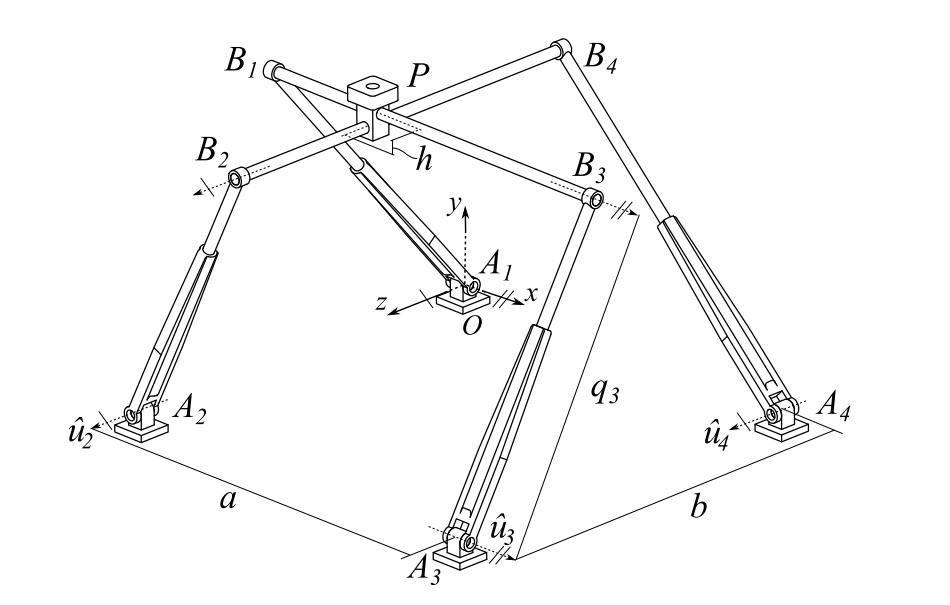
\includegraphics[width=0.50\linewidth ,height=0.4\columnwidth]{../lec_notes/figures/parallel_translational.png} \,\,
		&
		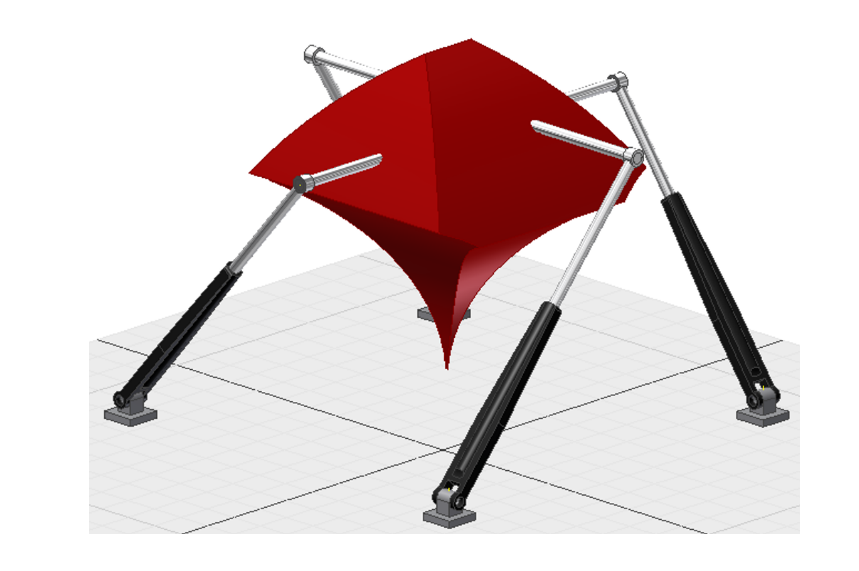
\includegraphics[width=0.48\columnwidth,height=0.4\columnwidth]{../lec_notes/figures/parallel_translational_workspace.png}
	\end{tabular}
	\caption{\textit{Left}: A Parallel Planar Robot Mechanism. \textit{Right:} Workspace of the mechanism.}
	\label{fig:para_mech}
\end{figure}

This robot has four RPRP-type kinematic chains. Three of these chains have their prismatic pair closest to the base; they serve as active joints. The fourth kinematic chain is completely passive.Points $B_1$ and $B_2$ are connected by a rod, which is perpendicular to the rod that connects points $B_2$ and $B_4$. Both rods ate connected to the moving platform by prismatic joints, which are separated from each other by a vertical offset $h$. Point $P = (P_x,P_y, P_z)$ is the interconnecting point for all the chains on the mobile platform and the top rods. Notice that the rotational axes of the revolute joints \ie, $\bm{\hat{u}}_i$ are parallel to the x-axes of joints 1 and 3; also, they are parallel to the z-axis for joints 2 and 4. 

There are many ways of solving this mobility problem. However, note that this mechanism has multiple closed loops and care must be taken when using the formulas we have introduced in our notes. Here, I will be using Gogu's method as proposed in ~\cite{Gogu}. It decomposes the mechanism into the different closed loops in order to properly analyze the mobility constraint. The mobility of the mechanism is 
%
\begin{align}
	\mathfrak{M} = \sum_{i=1}^{g} f_i - r
\end{align}
%
with $r$ being the number of joint parameters that lose independence after closing the loops of the mechanism. We define $r$ as 
%
\begin{align}
	r = \sum_{j=1}^{k}SH_j - SF  r_l
\end{align}
%
where $k$ is the number of closed-loops in the mechanism, $SH_j$ is the connectivity of the $j-th$ closed loop $H_j$ when separated from  the mechanism; SF is the overall connectivity of the mechanism and $r_l$ is the total number of parameters that lose independence in the closed loops. We may find the variables as follows
%
\begin{align}
	SH_j = \text{dim}(RH_j), \quad SF = \text{dim} (RF), \quad r_l = \sum_{j=1}^{k} r_l^{H_j}
\end{align}
%
where $RH_j$ is the velocity vector associated with the interest point $P$ in a closed loop $H_j$; RF is the resultant velocity vector formed from the intersection of $RH_j$ \ie $RF = RH_1 \cap RH_2 \ldots \cap RH_k$ and $r_l^{H_j}$ is the number of parameters that lose independence in the loop $H_j$. We define the variable $r_h^{H_j}$ as 
%
\begin{align}
	r_l^{H_j} = SG_1^{H_j} + SG_2^{H_j} - SF_{H_j} 
\end{align}
%
with $SG_i^{H_j}, i = 1,2$ being the connectivity of $G_i^{H_j}$ in $H_j$, whereas $SF_{H_j}$ is the loop's connectivity. We define
%
\begin{align}
	SG_i^{H_j} = \text{dim} \left(RG_{1,2}^{H_j}\right), \quad SF_{H_j} = \text{dim}\left(RF_{H_j}\right)
\end{align}
%
where $RG_i^{H_j}$ are the velocity vectors for $G_i^{H_j}$ and $RF_{H_j}$ is the resultant velocity vector formed by the intersection of the $RG_i^{H_j}$s.

For this mechanism, we have $g=14$ and $k=2$; Furthermore, we have $RH_1 = \{v_x \, v_y \, v_z \, \omega_x\}$ and $RH_2 = \{v_x\, v_y \, v_z \}$ so that the loops' connectivity are $SH_1 = 4$ and $SH_2 = 4$. Hence $RF = RH_1 \cap RH_2 = \{v_x \, v_y \, v_z\}$ and the mechanism's connectivity is thus $SF = \text{dim} (RF) = 3$.

If we disconnect the limbs, the velocity vector of $RG_1^{H_1} = RG_2^{H_1} = \{v_x \, v_z \, \omega_x\}$ and $RG_1^{H_2} = RG_2^{H_2} = \{v_x \, v_y \omega_z \}$, so that the connectivity of each limb is $SG_{1,2}^{H_1} = SG_{1,2}^{H_2} = 3$. Thus,
%
\begin{align}
	RF_{H_1} = RG_1^{H_1} \cap RG_2^{H_1} = \{ v_x \, v_z \, \omega_x\}, \quad RF_{H_2} = RG_1^{H_2} \cap RG_2^{H_2} = \{ v_x \, v_z \, \omega_z\}
\end{align}
%
so that $SG_{H_1} = SF_{H_2} = 3$.
%
Moreover, we see that $r_l^{H_1} = r_l^{H_2} = 3$ and $r_l = 6$. Thus, we have
%
\begin{align}
	r = SH_1 + SH_2 - SF + r_l = 11.
\end{align}
%
Since p = 14 and $f_i = 1$, we have 
%
\begin{align}
	\mathfrak{M} = 14 - 11 = 3. 
\end{align}
%
Hence, the mechanism has only 3 degrees of freedom. It is a planar parallel manipulator.

%\documentclass[]{article}


\usepackage{bm}
\usepackage{color}
\usepackage{graphicx}
\usepackage{mathrsfs}
\usepackage{microtype}
\usepackage{algpseudocode}
\usepackage[final]{pdfpages}
\usepackage{amssymb,amsthm,amsmath}

%opening
\title{Homework II}
\author{Dr. Olalekan Ogunmolu}

\theoremstyle{definition}
\newtheorem{definition}{Definition}[]
\newtheorem{theorem}{Theorem}[]
\newtheorem{example}{Example}
\newtheorem{homework}{Homework}
\newtheorem{solution}{Solution}
\definecolor{light-blue}{rgb}{0.30,0.35,1}
\definecolor{light-green}{rgb}{0.20,0.49,.85}
\definecolor{purple}{rgb}{0.70,0.69,.2}

\newcommand{\lb}[1]{\textcolor{light-blue}{#1}}
\newcommand{\bl}[1]{\textcolor{blue}{#1}}

\newcommand{\maybe}[1]{\textcolor{gray}{\textbf{MAYBE: }{#1}}}
\newcommand{\inspect}[1]{\textcolor{cyan}{\textbf{CHECK THIS: }{#1}}}
\newcommand{\more}[1]{\textcolor{red}{\textbf{MORE: }{#1}}}

% FYA
\newcommand{\cmt}[1]{{\footnotesize\textcolor{red}{#1}}}%{#2}
%\newcommand{\note}[1]{\cmt{Note: #1}}
%\newcommand{\todo}[1]{\textcolor{cyan}{TO-DO: #1}}
\newcommand{\review}[1]{\noindent\textcolor{red}{$\rightarrow$ #1}}
\newcommand{\response}[1]{\noindent{#1}}
\newcommand{\stopped}[1]{\color{red}STOPPED HERE #1\hrulefill}

%Text commands
\newcounter{mnote}
\newcommand{\marginote}[1]{\addtocounter{mnote}{1}\marginpar{\themnote. \scriptsize #1}}
\setcounter{mnote}{0}
% \newcommand{\comment}[1]{}
\newcommand{\ie}{$i.e.$\ }
\newcommand{\eg}{e.g.\ }
\newcommand{\cf}{c.f.\ }
\newcommand{\yes}{\checkmark}
\newcommand{\no}{\ding{55}}

%Reference commands
\newcommand{\flabel}[1]{\label{fig:#1}}
\newcommand{\seclabel}[1]{\label{sec:#1}}
\newcommand{\tlabel}[1]{\label{tab:#1}}
\newcommand{\elabel}[1]{\label{eq:#1}}
\newcommand{\alabel}[1]{\label{alg:#1}}
\newcommand{\fref}[1]{\cref{fig:#1}}
\newcommand{\sref}[1]{\cref{sec:#1}}
\newcommand{\tref}[1]{\cref{tab:#1}}
\newcommand{\eref}[1]{\cref{eq:#1}}
\newcommand{\aref}[1]{\cref{alg:#1}}

\newcommand{\bull}[1]{$\bullet$ #1}
\newcommand{\argmax}{\text{argmax}}
\newcommand{\argmin}{\text{argmin}}
\newcommand{\mc}[1]{\mathcal{#1}}
\newcommand{\bb}[1]{\mathbb{#1}}


\def\tidx{t}
%\def\comment
%\def\value{V}
% from https://www.cs.jhu.edu/~jason/advice/write-the-paper-first.html
\newcommand{\Note}[1]{}
\renewcommand{\Note}[1]{\hl{[#1]}}  % comment out this definition to suppress all Notes
%\algnewcommand\algorithmicforeach{\textbf{for each}}
%\algdef{S}[FOR]{Foreach}[1]{\algorithmicforeach\ #1\ \algorithmicdo} %

%\newcolumntype{M}[1]{>{\centering\arraybackslash}m{#1}}
\def\coriolis{\textbf{\textit{C}}}
\def\massinertia{\textbf{\textit{M}}}
\def\torque{\bm{\tau}}
\def\frictionvec{\textbf{\textit{f}}}
\def\Smat{\textbf{\textit{S}}}
\def\Bmat{\textbf{\textit{B}}}
\def\wheelrad{\textbf{\textit{r}}}

\def\stateweight{\textbf{\textit{w}}_x}
\def\actionweight{\textbf{\textit{w}}_u}
\def\advactionweight{\textbf{\textit{w}}_v}

%Thesis defs
%\def\upchi{\textchi}
\def\kau{\mc{K}}
\def\particle{\bm{x}}
\def\deformationgrad{\textbf{F}}
\def\refconf{\bm{\upchi}_0}
\def\refconfbody{\mathscr{B}_0}
\def\conf{\bm{\upchi}}
\def\currconf{\bm{\upchi}}
\def\Eulerian{\mc{E}}
\def\cauchystress{\bm{\sigma}}
\def\stresscomp{\sigma}
\def\currconfbody{\mathscr{B}}
\def\materialresponse{\textbf{G}}
\def\orthoggroup{{\textit{SO}}(3)}
\def\liegroup{{\textit{SE}}(3)}
\def\liealgebra{\mathfrak{se}(3)}
\def\identity{\textbf{I}}
\newcommand{\trace}[1]{\textbf{tr}(#1)}
\def\leftcauchy{\textbf{B}}
\def\rightcauchy{\textbf{C}}
\def\fiber{\textbf{dx}}

\def\dof{\text{DOF }}
\def\dofs{\text{DOFs }}
\def\reline{\mathbb{R}}
\def\curve{\deformationgrad}
\def\twist{{\xi}}
\def\contactforce{\tilde{F}}
\def\contactforcecomp{f}
\def\gaussianmap{\textbf{}n}
\def\contacttorquecomp{\tau}
\def\wrt{with respect to }
\def\curveparam{\position}
\def\basis{\bm{e}}
\def\pose{{g}}
\def\selmap{{B}}
\def\manipmap{{G}}
\def\jacob{\bm{J}}
\def\normal{\bm{n}}
\def\position{\textbf{r}}
\def\deformationgradcur{\textbf{H}}
\def\eulerianvel{\textbf{v}(\position, t)}
\def\headparam{\zeta}
\def\strain{\mathrm{\Psi}}
\def\strainiso{\mathrm{\Psi_{\text{iso}}}}
\def\strainfiber{\mathrm{\Psi_{\text{mesh}}}}

% mechanism defs
\def\wallthickness{1cm}
\def\sorodiam{9 cm}
\def\sorodiamdim{5-6.25cm}

% inline macros
\newcommand{\putsoro}[2]{\includegraphics[width=.45\columnwidth,height=#2\columnwidth]{../../../PhDThesis/figures/#1}}
\newcommand{\sorowidth}{.35}


%\newtheorem{theorem}{Theorem}[]
%\newtheorem{example}{Example}
%\newtheorem{homework}{Homework}


\begin{document}

\maketitle


\noindent 
\begin{homework}
	What is the geometric meaning of equation 3.1.6 on a twist axis to you. Define \textit{pure rotation} and a \textit{pure translation} in terms of equation 3.1.6\footnote{Figure out how they correspond to zero pitch and infinite pitch twists.}. 
\end{homework} 

\begin{solution}
	Twists and pitches of twists.
	\begin{enumerate}
		\item The pitch of the twist is the ratio of the magnitude of a point on the axis of the twist to the magnitude of the angular velocity about the axis of the twist. By this, we see that the pitch of the twist is the unit velocity traveled along the axis of the twist.
		%
		\item A pure rotation occurs when the numerator of equation 3.1.6 is zero \ie when a point travels only in the angular velocity direction of the twist axis; this is called a zero pitch twist.
		%
		\item A pure translation occurs when the right hand side of 3.1.6 is infinite. This corresponds to an infinite pitch twist \ie a point on the twist axis only travels along the linear velocity direction of the twist axis.
	\end{enumerate}
\end{solution}

\noindent 
\begin{homework}
	A unit screw, twist or wrench is one where the magnitude of the screw, twist or wrench is $1$.  
	\begin{enumerate}
		\item  What is the geometric meaning of a unit screw to you? 
		\item Consult the identified reference materials and explain what a reciprocal screw is in no more than five sentences.
	\end{enumerate}
\end{homework}

\noindent \begin{solution}
	Here is a geometric meaning of the screw:
	%
	\begin{enumerate}
		\item 
		Imagine a nut fitted upon a mechanical screw. As we tighten the nut around the threads of the screw, there exists a rectilinear distance by which the screw travels into the nut. This rectilinear distance is called the \textit{pitch} of the screw. Thus, the pitch is a linear magnitude. When a nut is rotated about the threads of a screw, the rectilinear distance by which the nut moves when rotated through a particular angle is the product of the pitch and the the circular measure of the angle. \textit{A screw then may be geometrically seen as a straight line with which a definite linear magnitude, \ie the pitch, travels in space.}
		
		Often with twist and wrenches, we wish to associate a magnitude other than 1 so that there are $\infty^6$ different twists and wrenches if we consider their magnitudes as well. With this interpretation we can think of a unit screw as defining only an axis and a pitch. Then we can think of a given magnitude as defining a twist (if its units are rotation/time) or a wrench (if its units are force) acting along the screw. In both cases the pitch is expressed in length units. These six-spaces of (infinitesial) twists or wrenches can be considered to be vector spaces in that they are closed under vector addition and scalar multiplication.
		%
		\item \textbf{Reciprocal Screws:} Suppose a body is free to twist about a screw $x$ and that body is in equilibrium, while being acted upon by a wrench on another screw $\chi$; we can extend this logic and infer that a body that is free to rotate about the screw $\chi$ will be in equilibrium, while being acted upon by a wrench on a screw $x$. By the principle of virtual velocities, if the body is in equilibrium the work done in a small displacement against external forces must be zero with the virtual coefficient vanishing. %Suppose $p_\alpha$ represent the pitch of a screw $\alpha$ 
		\textit{A pair of screws are reciprocal when their virtual coefficient is zero.}
	\end{enumerate}
\end{solution}


\noindent 
\begin{homework}
	Given a matrix $\hat{m} \in so(3)$, suppose that the following relation holds,
	%
	\begin{align}
	\hat{m}^2 = m m^T - \|m\|^2 \identity \\
	%
	\hat{m}^3 = - \|m\|^2 \hat{m}
	\end{align}
	%
	with the fact that higher powers of $\hat{m}$ can be recursively found. Utilizing this lemma along with $m =\omega \theta$, and $\|\omega\| = 1$, show that 
	%
	\begin{align}
	e^{\hat{\omega}\theta}  = \identity + \hat{\omega} \sin \theta + \hat{\omega}^2(1 - \cos \theta).
	\label{eq:rodrigues}
	\end{align}
\end{homework} 

\begin{solution}
	First recall that we can expand $e^{\hat{\omega}\theta}$ using Taylor series so that 
	%
	\begin{align}
		e^{\hat{\omega}\theta} = \identity + \theta \hat{\omega} + \frac{\theta^2}{2!}\hat{\omega}^2 + \frac{\theta^3}{3!}\hat{\omega}^3 + \frac{\theta^4}{4!}\hat{\omega}^4 + + \frac{\theta^5}{5!}\hat{\omega}^5 + \frac{\theta^6}{6!}\hat{\omega}^6 + \frac{\theta^7}{7!}\hat{\omega}^7 + \cdots
	\end{align}
	%
	Rewriting, we find that
	%	
	\begin{align}
	e^{\hat{\omega}\theta} = \identity + \hat{\omega} \left(\theta + \frac{\theta^3}{3!}\hat{\omega}^2  + \frac{\theta^5}{5!}\hat{\omega}^4 + \frac{\theta^7}{7!}\hat{\omega}^6  + \cdots \right)  +
	% 
	\hat{\omega}^2 \left( \frac{\theta^2}{2!} + \frac{\theta^4}{4!}\hat{\omega}^2 + + \frac{\theta^6}{6!}\hat{\omega}^4  + \cdots \right).
	\label{eq:exp_expand}
	\end{align}
	%
	Since we have from the lemma that 
	%
	\begin{subequations}
		\begin{align}
		\hat{\omega}^2 = \omega \omega^T - \|\omega\|^2 \identity  \\
		%
		\hat{\omega}^3 = - \|\omega\|^2 \hat{\omega}
		\end{align}
	\end{subequations}
	%
	we may write \eqref{eq:exp_expand} as 
	%
	\begin{align}
	e^{\hat{\omega}\theta} &= I + \hat{\omega} \left(\theta + \frac{\theta^3}{3!}\left(\omega \omega^T - \|\omega\|^2 \identity\right)  + \frac{\theta^5}{5!}\left(\omega \omega^T - \|\omega\|^2 \identity\right)^2 + \frac{\theta^7}{7!}\left(\omega \omega^T - \|\omega\|^2 \identity\right)^3  + \cdots \right) \nonumber \\
	&\quad +
	% 
	\hat{\omega}^2 \left( \frac{\theta^2}{2!} + \frac{\theta^4}{4!}\left(\omega \omega^T - \|\omega\|^2 \identity \right) + \frac{\theta^6}{6!}\left(\omega \omega^T - \|\omega\|^2 \identity \right)^2  + \frac{\theta^8}{8!}\left(\omega \omega^T - \|\omega\|^2 \identity\right)^4 + \cdots \right) \nonumber \\
	%
	&= \identity + \hat{\omega} \left(\theta - \frac{\theta^3}{3!}\hat{\omega}^2  + \frac{\theta^5}{5!}\hat{\omega}^4 - \frac{\theta^7}{7!}\hat{\omega}^6  + \cdots \right)  +
	% 
	\hat{\omega}^2 \left( \frac{\theta^2}{2!} - \frac{\theta^4}{4!}\hat{\omega}^2 + + \frac{\theta^6}{6!}\hat{\omega}^4  + \cdots \right)
	\label{eq:exp_lemma}
	\end{align}
	%
	Recall from trigonometric identities that 
	%
	\begin{subequations}
		\begin{align}
		\sin \theta &= \theta - \frac{\theta^3}{3!}  + \frac{\theta^5}{5!} - \frac{\theta^7}{7!}  + \cdots  \nonumber \\
		%
		\cos \theta		&= 1 - \frac{\theta^2}{2!} + \frac{\theta^4}{4!} - \frac{\theta^6}{6!} + \cdots
		\end{align}
	\end{subequations}
%
Therefore, \eqref{eq:exp_lemma} becomes 
%
	\begin{align}
		e^{\hat{\omega}\theta} &= \identity + \hat{\omega} \sin \theta + \hat{\omega}^2\left(1-\cos \theta \right)
	\end{align}
	%
	where we have used the identities $\hat{\omega}^2 = -1$ and $\hat{\omega}^4 = 1$ etc.
\end{solution}

\end{document}

%
\noindent 
\begin{homework}
	Verify that $R_{ij} = R_{ji}^{-1} \equiv R_{ji}^T$. Furthermore, verify that the determinant of the rotation matrix is $\pm1$ \ie $det R = \pm1$.
\end{homework}

\begin{solution}
	We have from equation 3.4.9 in our notes that
%
\begin{align}
R_{ji} &= 	\begin{bmatrix}
	\bm{x}_j \cdot \bm{x}_i & \bm{y}_j \cdot \bm{x}_i & \bm{z}_j \cdot \bm{x}_i \\
	%
	\bm{x}_j \cdot \bm{y}_i & \bm{y}_j \cdot \bm{y}_i & \bm{z}_j \cdot \bm{y}_i \\
	%
	\bm{x}_j \cdot \bm{z}_i & \bm{y}_j \cdot \bm{z}_i & \bm{z}_j \cdot \bm{z}_i 
	\end{bmatrix} 
	\label{eq:rot}
	\end{align}
	%
	and that
	%
\begin{align}
	R_{ij}^T & = 
	\begin{bmatrix}
	\bm{x}_j \cdot \bm{x}_i & \bm{x}_j \cdot \bm{y}_i  & \bm{x}_j \cdot \bm{z}_i \\
	%
	\bm{y}_j \cdot \bm{x}_i & \bm{y}_j \cdot \bm{y}_i & \bm{y}_j \cdot \bm{z}_i \\
	%
	\bm{z}_j \cdot \bm{x}_i & \bm{z}_j \cdot \bm{y}_i  & \bm{z}_j \cdot \bm{z}_i 
	\end{bmatrix}
	\end{align}
	%
	Inspecting the rows of $R_{ij}$ and $R_{ij}^T$, the dot products between the respective vector elements are simply the cosine of the angles between them \ie $p_j \cdot p_i = cos \theta$, where $\theta$ is the angle between the vectors $p_j$ and $p_i$. Evaluating, it follows that $R_{ij}^T = R_{ij}$. Similarly, we know that a matrix $X$ is invertible if there exists a matrix $B$ such that
	%
	\begin{align}
		AB = BA = \identity_n
	\end{align}
	%
	where $I_n$ is an $n \times n$ matrix. In this case, we have that 
	%
	\begin{align}
	R_{ij} R_{ij}^T = R_{ij}^T R_{ij} = \identity_3.
	\end{align}
	%
	It follows that, 
	%
	\begin{align}
	R_{ij} = \dfrac{1}{R_{ij}^T} = \dfrac{1}{R_{ij}} 
	\end{align}
	%
	or 
	\begin{align}
	R_{ij} = R_{ij}^{-T} = R_{ij}^{-1}. 
	\end{align}
	%
	Hence, 
	\begin{tcolorbox}[title=QED]
		$R_{ij} = R_{ji}^{-1} \equiv R_{ji}^T$.
	\end{tcolorbox}.
\end{solution}


\begin{homework}
	Compose the rotation matrix in three dimensions where all axes of the inertial frame are rotated by an angle $\beta$ around each of the $x_0$, $y_0$ and $z_0$ axes respectively using the foregoing logic. In addition, for each transformation, verify that (1) $R_{e, 0} = I$\footnote{In your notes, this was written as $R_{e, \beta}$. You will not be penalized if you could not arrive at the right solution because of this mistake.} where $e$ is the axes about which we are rotating and $\beta$ is the angle of rotation, (2) the composition of rotations about the angles $\beta$ and $\alpha$ in a successive manner implies that $R_{z, \beta}, R_{z, \alpha} = R_{z, \beta + \alpha}$, and (3) ${(R_{z, \beta})}^{-1} = R_{z, -\beta}$. Bonus points will be awarded for cool 3D visualizations.
\end{homework} 

\begin{solution}
	In three dimensions, a rotation angle of $\beta$ around the principal axes of the moving frame  $x_0, y_0, z_0$, gives the rotation matrix
	%
	\begin{align}
	\begin{bmatrix}
	\bm{x}_1 \cdot \bm{x}_0 & \bm{y}_1 \cdot \bm{x}_0   &   \bm{z}_1 \cdot \bm{x}_0  \\
	%
	\bm{x}_1 \cdot \bm{y}_0    & \bm{y}_1 \cdot \bm{y}_0   &  \bm{z}_1  \cdot  \bm{y}_0 \\
	%
	 \bm{x}_1\cdot  \bm{z}_0   &   \bm{y}_1 \cdot \bm{z}_0  &  \bm{z}_1 \cdot \bm{z}_0
	\end{bmatrix} 
	%
	\end{align}
	%	
	A rotation about $x$ by $\beta$ gives,
	%
	\begin{align}
	R_{x_0, \beta} = \begin{bmatrix}
	1 & 0   &  0  \\
	%
	0   & \cos \beta   &  -\sin \beta  \\
	%
	0  &  \sin \beta  &  \cos \beta 
	\end{bmatrix},
	\label{eq:rbx}
	\end{align}
	%
	a rotation about $y_0$ by $\beta$ gives,
	%
	\begin{align}
	R_{y_0, \beta} = \begin{bmatrix}
	\cos \beta & 0   &  \sin \beta   \\
	%
	0   &  1   &  0 \\
	%
	-\sin \beta  &  0  &  \cos \beta 
	\end{bmatrix}
	\label{eq:rby}
	\end{align}
	%
	and a rotation about $z_0$ by $\beta$ gives,
	%
	\begin{align}
	R_{z_0, \beta} = \begin{bmatrix}
	\cos \beta & -\sin \beta    &  0  \\
	%
	\sin \beta    &  \cos \beta   &  0 \\
	%
	0 &  0  &  1 
	\end{bmatrix}.
	\label{eq:rbz}
	\end{align}
	%
	Substituting $0$ for $\beta$ in \eqref{eq:rbx}, \eqref{eq:rby}, and \eqref{eq:rbz}, we have
	%
	\begin{align}
		R_{x_0, \beta} = R_{\beta, y_0} = R_{\beta, z_0} = \begin{bmatrix}
		1 & 0   &  0  \\
		%
		0    &  1   &  0 \\
		%
		0 &  0  &  1 
		\end{bmatrix}.
	\end{align}
	
	The composition of rotations about the angles $\beta$ and $\alpha$ in a successive manner implies that $R_{z, \beta}  R_{z, \alpha} = R_{z, \beta + \alpha}$
	
	\noindent \textbf{Proof}: 
	\begin{align}
		R_{\beta, z_0} R_{\alpha, z_0}  &= \begin{bmatrix}
		\cos \beta & -\sin \beta    &  0  \\
		%
		\sin \beta    &  \cos \beta   &  0 \\
		%
		0 &  0  &  1 
		\end{bmatrix} \, \begin{bmatrix}
		\cos \alpha & -\sin \alpha    &  0  \\
		%
		\sin \alpha    &  \cos \alpha   &  0 \\
		%
		0 &  0  &  1 
		\end{bmatrix} \\ 
		%
	R_{\beta, z_0} R_{\alpha, z_0}	&= \begin{bmatrix}
		c_\alpha c_\beta -s_\alpha s_\beta & c_\alpha s_\beta -c_\beta s_\alpha    &  0  \\
		%
		c_\alpha s_\beta + s_\alpha c_\beta    &  c_\alpha c_\beta - s_\alpha s_\beta  &  0 \\
		0 & 0 & 1
		\end{bmatrix} .
	\end{align}
	%
	or 
	\begin{align}
	R_{\beta, z_0} R_{\alpha, z_0}	&= \begin{bmatrix}
		\cos(\alpha + \beta) & -\sin(\alpha + \beta)    &  0  \\
		%
		\sin(\alpha + \beta)     &  \cos(\alpha + \beta)  &  0 \\
		0 & 0 & 1
	\end{bmatrix} .
	\label{eq:rot_a_then_b}
\end{align}

Now, we find that 
%
\begin{align}
	R_{z, \beta + \alpha} = \begin{bmatrix}
	\cos(\alpha + \beta) & -\sin(\alpha + \beta)    &  0  \\
	%
	\sin(\alpha + \beta)     &  \cos(\alpha + \beta)  &  0 \\
	0 & 0 & 1
	\end{bmatrix}.
	\label{eq:rot_a_plus_b}
\end{align}
%
Since \eqref{eq:rot_a_then_b} = \eqref{eq:rot_a_plus_b}, the supposition is confirmed.

\noindent \textbf{Prove that ${(R_{z, \beta})}^{-1} = R_{z, -\beta}$}:
%
We have from \eqref{eq:rbz} that
%
\begin{align}
R_{z, -\beta} = \begin{bmatrix}
\cos(-\beta )& -\sin (-\beta)    &  0  \\
%
\sin (-\beta)    &  \cos (-\beta)   &  0 \\
%
0 &  0  &  1 
\end{bmatrix} = \begin{bmatrix}
\cos(\beta )& \sin (\beta)    &  0  \\
%
-\sin (\beta)    &  \cos (\beta)   &  0 \\
%
0 &  0  &  1 
\end{bmatrix}.
\end{align}

Now, $(R_{z, \beta})^{-1}$ = $(R_{z, \beta})^T$ so that 
%
\begin{align}
	R_{z, \beta}^T = \begin{bmatrix}
	\cos \beta & \sin \beta    &  0  \\
	%
	-\sin \beta    &  \cos \beta   &  0 \\
	%
	0 &  0  &  1 
	\end{bmatrix}.
\end{align}
%
The equivalence of the two preceding equations prove our case. (QED)
\end{solution}

\begin{figure}[tb!]
	\centering
	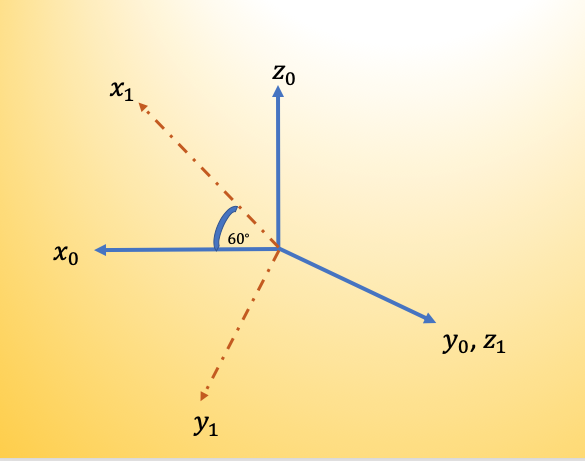
\includegraphics[width=.8\columnwidth]{../lec_notes/figures/two_frames.png}
	\caption{Relative orientation between two frames.}
	\label{fig:two_frames}
\end{figure}


\noindent 
\begin{homework}
	For the two frames shown in \autoref{fig:two_frames}, determine the rotation matrix between them. In addition, explain the difference between rotating about a \textit{current frame} and rotating about a \textit{fixed frame}\footnote{See sections 2.4.1 and 2.4.2 of Spong's book.}. In particular, when is it necessary to carry out a \textit{pre-multiplication} and when is it necessary to carry out a \textit{post-multiplication} when transforming points or vectors about coordinate frames?
\end{homework}

\begin{solution}
	From the given figure, observe that the $x_0$ axis was rotated counterclockwise by $60^\circ$ from the horizontal. To find the rotation matrix between the two frames, we can project the unit vectors $x_1, y_1, z_1$ onto $x_0, y_0, z_0$ to generate the coordinates of $x_1, y_1, z_1$ in the $x_0, y_0, z_0$ frame. We therefore have
	%
	\begin{align}
		x_1 = \begin{bmatrix}
		\frac{1}{2} 
		\\
		0
		\\
		\frac{\sqrt{3}}{2}
		\end{bmatrix}, \quad
		%
		y_1 = \begin{bmatrix}
		\frac{\sqrt{3}}{2}
		\\
		0
		\\
		-\frac{\sqrt{3}}{2}
		\end{bmatrix},  \quad
		%
		z_1 = \begin{bmatrix}
		0
		\\
		1
		\\
		0
		\end{bmatrix}
	\end{align}
\end{solution}


\noindent 
\begin{homework}
	For the robot manipulator we are using in this class, suppose that you have the following point in the base frame of the robot, $q_o = [-2, 3, 1]$. Furthermore, suppose that the joint angles for all six joints are respectively $\{-90, 60, 30, 45, 90, 125 \}$, transform the point $q_0$ in the base frame to a coordinate frame on the sixth joint.
\end{homework}

\begin{solution}
Since we changed the robot we are using, this homework is rendered moot and you will not be graded for it.
\end{solution}

Consider the composition of rotations of \autoref{fig:compoz} where we first rotate by an angle $\theta$ about the $x$ axis and then rotate about an angle $\psi$ about the $z$ axis. The rotation matrix can be composed as 
%
\begin{figure}[tb!]
	\centering
	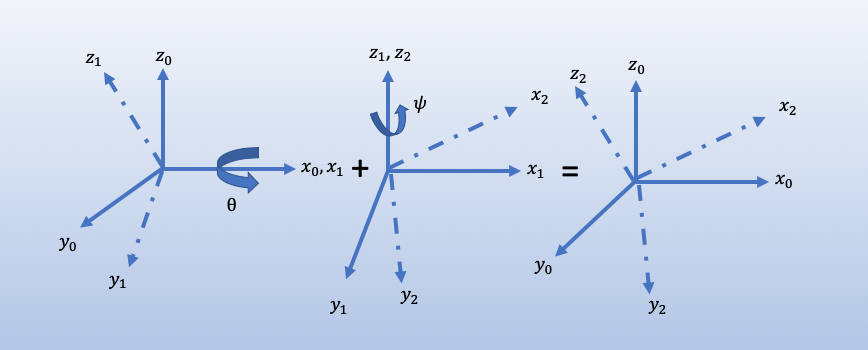
\includegraphics[width=\columnwidth]{../lec_notes/figures/compoz.png}
	\caption{Illustration of composition of rotations about a \textbf{current axis}.}
	\label{fig:compoz}
\end{figure}
%
\begin{align}
R &= R_{x, \theta} R_{z, \psi} 
%
&= \left(\begin{array}{ccc}
1 & 0 & 0 \\
0 & c_\theta & -s_\theta \\
0 & s_\theta & c_\theta
\end{array}\right) 
%
\cdot
%
\left(\begin{array}{ccc}
c_\psi & -s_\psi & 0 \\
s_\psi & c_\psi & 0 \\
0 & 0 & 1
\end{array}\right)
\end{align}
%
\begin{align}
R	&= \left(\begin{array}{ccc}
	c_\psi & -s_\psi & 0 \\
	c_\theta s_\psi & c_\theta c_\psi &  -s_\theta \\
	s_\theta s_\psi & s_\theta c_\psi & c_\theta 
	\end{array}\right)
\end{align}
Notice how the order of multiplication is carried out, owing to the axis about which we are making the transformation. 

\noindent 
\begin{homework}
	Carry out the transformation above in reverse order. What do you notice?
\end{homework} 

\begin{solution}
	Reversing the order of transformation reveals that
	\begin{align}
 R_{z, \psi} R_{x, \theta}=
	%
	\left(\begin{array}{ccc}
	c_\psi & -s_\psi & 0 \\
	s_\psi & c_\psi & 0 \\
	0 & 0 & 1
	\end{array}\right)
	%
	\cdot
	%
	 \left(\begin{array}{ccc}
	1 & 0 & 0 \\
	0 & c_\theta & -s_\theta \\
	0 & s_\theta & c_\theta
	\end{array}\right) 
	\end{align}
	%
	\begin{align}
		R &=  R_{z, \psi} R_{x, \theta} = \left(\begin{array}{ccc}
		c_\psi & -c_\theta s_\psi & s_\psi s_\theta \\
		s_\psi & c_\psi c_\theta  & - c_\psi s_\theta \\
		0 & s_\theta & c_\theta
		\end{array}\right)
	\end{align}
	\ie $R_{x, \theta} R_{z, \psi} = (R_{x, -\theta} R_{z, -\psi})^T $
\end{solution}
%
which goes to show that reversing the order of rotations is tantamount to reversing the order of angle rotations and then taking the transpose of the ensuing result. 

% ---- Bibliography ----
\providecommand\BIBentryALTinterwordstretchfactor{2.5}
\bibliographystyle{IEEEtran}
\bibliography{../../Papers/SRS/Continuum/biblio}	
\end{document}	